\section{Approaches}

This section discusses the optimization of the enumerators with two different approaches in each case. In addition, a third approach evaluated is the avoidance of scanning unsupported services. 

\subsection{Use information of a former service scan}

This approach aims to reuse information from one enumerator in a later enumerator within the same scan. This will be applied to the RCEnumerator.

The Routine Control service is used by the client to execute a defined sequence of steps and obtain any relevant results \cite{iso14229}. For a quick overview of the service a simplified code snippet of the Scapy implementation is used.

\begin{samepage}
\begin{minted}{python}
class UDS_RC(Packet):
    routineControlTypes = {
        1: 'startRoutine',
        2: 'stopRoutine',
        3: 'requestResults'
    }
    fields_desc = [
        ByteEnumField('routineControlType', 0, routineControlTypes),
        XShortField('routineIdentifier', 0)
    ]
\end{minted}
\end{samepage}

The routineControlType field specifies what to do with a routine. Possible are starting, stopping and requesting the results. To specify which routine is to be controlled, there is the routineIdentifier field. Hence, there are three control types, and because the identifier is a short field, there are 2\textsuperscript{16} identifiers. This leads to the following formula, showing how many requests are generated for a UDS scan:
\[f(n)=3 * 2^{16} * n\]
wherin $n$ stands for the number of detected states.

The current RCEnumerator does exactly this, it generates the full range for each states. That's what needs to be reduced. Its current behavior is illustrated in \autoref{fig:rc-behavior-current}. The green areas show the scanned regions.

\begin{figure}[h]
    \centering
    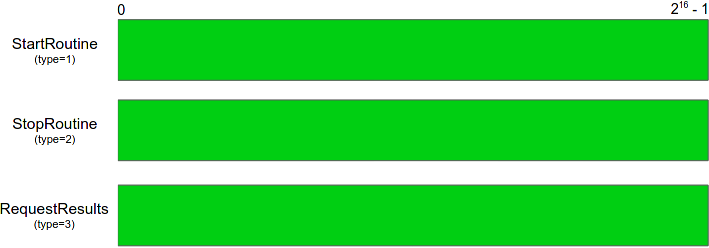
\includegraphics[width=1\textwidth]{rc-behavior-current}
    \caption{Behavior of the current RCEnumerator implementation.}
    \label{fig:rc-behavior-current}
\end{figure}

As a first step to find a way to apply the approach to the RCEnumerator, the distribution of the identifiers is visualized grouped by the type as a histogram in \autoref{fig:rc-distribution}.

% TODO: maybe to attachments
\begin{figure}[h]
    \centering
    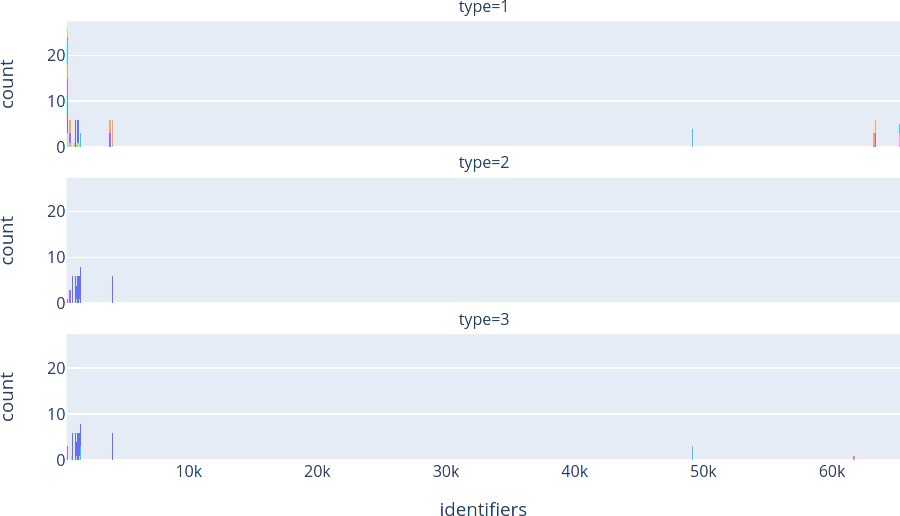
\includegraphics[width=1\textwidth]{rc-distribution}
    \caption{Distribution of the RC identifiers. A color is one ECU.}
    \label{fig:rc-distribution}
\end{figure}

It can be seen that if an identifier is available in Type1, it is likely that this identifier also occurs in Type2. Consequently, if an identifier does not respond positively in Type1, it is also very unlikely that it will respond in Type2 or Type3. This appearance is used to reduce the scan range for this service.

The new behavior starts with scanning all 2\textsuperscript{16} identifiers with Type1. So, 2\textsuperscript{16} is the minimum number of requests for each state with the new behavior. Only the identifiers, which led to a positive response, are scanned with Type2 and Type3 as well. Moreover, it was observed that there seems to be a locality effect for the identifiers. Thus, if an identifier with Type1 is answered positively, scanning nearby identifiers instead of just that identifier will result in higher coverage. What needs to be found out is the block size which leads to the best coverage, while maintaining an appropriate speed-up.

The limits of the speed-up are defined as following:
\[ 0\ \% \ \leq\  s(n)\  \leq 66.\overline{66}\ \% \quad \forall \  n \in \left\{0, 1, ..., 2^{16} * 3\right\} \]
%\[ 0\  \ \leq\  s(n)\  \leq \frac{2}{3} \quad \forall \  n \in \left\{0, 1, ..., 2^{16 * 3}\right\} \]
wherin $s$ is the speed-up function and $n$ the number of generated requests.

The reason for the upper limit of $66.\overline{66}$ \% of this approach for this enumerator is because the first third is type1 and this is always scanned completely.

To find out the best value, scans with different block sizes are simulated. For a quick simulation another observation is used. If one identifier is available in one state, it is likely to be available in the other states too. Thus, the states are ignored in the simulation, which improves the performance by a multiple, while it is still very close to the real ECUs. The simulation only uses information gathered from the real ECUs as described in \autoref{sec:data-gathering}. Specifically, the required information is extracted from the generic.log file.

As described, the simulation starts with getting all identifiers which have been positively answered of the currently simulated ECU. Subsequently, these identifiers are expanded to blocks of the size from 1 to 200. Overlapping blocks are resolved to one continuous space. With these blocks the coverage and the number of requests can be calculated. The number of requests can be converted to the speed-up. The results are averaged.
The blocks are expanded in both directions. So, for example, if the identifier 500 has been answered positively and the block size is 100, it leads to range from 400 to 600. A simulation was also run with expanding individual identifiers in one direction only, which yielded very similar results. Thus, it was left with the expansion in both directions. 
The following pseudocode shows the procedure more clearly.

\begin{samepage}
\begin{minted}{python}
coverages = []
speedups = []
for block_width in range(200):
    coverages_block = []
    speedups_block = []
    for ecu in ecus:
        ids_type1 = get_type1_ids(ecu)
        to_scan = ids_to_block(ids_type1, block_width)
        coverages_block.append(get_coverage(ecu, to_scan))
        count_requests = len(to_scan)
        speedups_block.append(get_speedup(ecu, count_requests))
    coverages.append(avg(coverages_block))
    speedups.append(avg(speedups_block))
\end{minted}
\end{samepage}

The results of this simulation are plotted in \autoref{fig:rc-simulation-result}. The speed-up is linear to the block size. That makes sense, because the larger the blocks are, the more requests are generated, since the positively answered identifiers are independent of the block size. The block size of zero represents the results without using the locality effect. The maximum difference in coverage of with and without locality effect are 22\%, even though the maximum speed-up difference is only 1\%.

\begin{figure}[h]
    \centering
    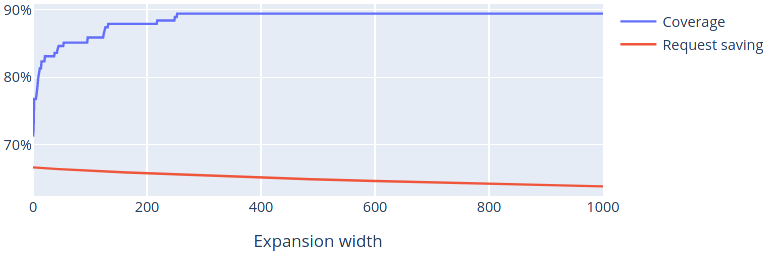
\includegraphics[width=0.7\textwidth]{rc-simulation-result}
    \caption{Simulation result for the RC service.}
    \label{fig:rc-simulation-result}
\end{figure}

Since the speed-up is high for each simulated block size, the highest coverage was chosen which starts with block size \textbf{132}. Hence, this value is the chosen and implemented block size.


\subsection{Reduction of scan range}


\subsection{Avoid the scan of unsupported services}
